% style du document
\documentclass{book}
% réglage des marges
\usepackage[papersize={12.5cm,17.7cm},margin=1.2cm,includehead,includefoot]{geometry}
% encodage du texte
\usepackage[utf8]{inputenc}
% dictionnaire
\usepackage[francais]{babel}
% pour les poèmes
\usepackage{verse}
% pour les URLs
\usepackage{hyperref}
% pour la police d'écriture
% run updmap to update the fonts map
\usepackage{kpfonts}
% pour l'image dans le titre
\usepackage{titlepic}
% pour les images
\usepackage{graphicx}
% pour modifier les chapitres
\usepackage{titlesec}
\titleformat{\chapter}[display]{\normalfont\huge\bfseries}{\chaptertitlename\ \thechapter}{20pt}{\Huge}
\titlespacing*{\chapter}{0pt}{0pt}{40pt}
% pour le filigrane
%\usepackage{draftwatermark}
% pour la profondeur du chiffrage
\setcounter{secnumdepth}{0}
% pour le comptage des poèmes
\newcounter{compteur}
\newcommand{\numero}{\Roman{compteur}.~}
% pour les headers
\renewcommand{\chaptermark}[1]{\markboth{\MakeUppercase{\hfill #1 \hfill}}{}}
\renewcommand{\sectionmark}[1]{\markright{\MakeUppercase{\hfill #1 \hfill}}{}}
% pour les auteurs
\newcommand{\attrib}[1]{\nopagebreak{\raggedleft\footnotesize #1\par}}


\title{\Huge{\textsc{l'Orbe}}\\\small{\emph{recueil de poésie}}\\\small{\textsc{textes de 2003 à 2008}}
}

\author{\textsc{Kévin Guignard}}
\titlepic{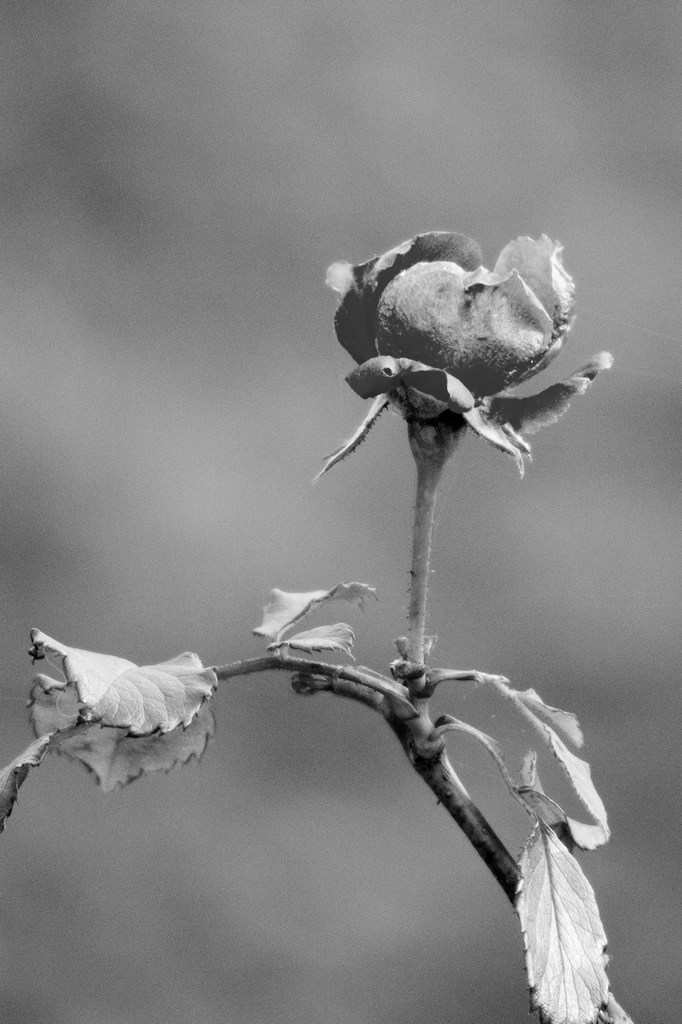
\includegraphics[width=0.4\textwidth]{picture.jpg}}
\date{}
\hypersetup{
	pdftoolbar=false,
	pdfmenubar=false,
	pdffitwindow=true,
	pdfborderstyle = {/S/U/W 1}
}

\begin{document}

\maketitle
~
\vfill
\begin{center}
\footnotesize{\copyright~Kévin Guignard, 2013 et 2016.\\Tous droits réservés.}
\end{center}

%%%%%%%%%%%%%%%%%%%%%%%%%%%%%
% PREFACE
%%%%%%%%%%%%%%%%%%%%%%%%%%%%%
\chapter*{Préface}
Ce recueil de poèmes est composé de deux parties, conçues à l'origine comme des recueils indépendants et eux-même divisés en trois chapitres ; la première intitulée \emph{Le Schisme du soir} a été écrite entre 2003 et 2005 pendant mes années lycées ; la seconde nommée \emph{L'Amour en doute} a été écrite entre 2005 et 2008 lorsque j'étais en faculté. Bien que les premiers poèmes soit de mon propre aveu brouillons et enfantins, il m'est apparu nécessaire de les laisser pour en comprendre le dénouement : \emph{L'Orbe} est un chemin de vie, une évolution de pensées. %Quant au court récit qui lui fait suite, \emph{La Légende de Tethys}, il s'agit d'un conte fantastique écrit entre 2008 et 2011 puis totalement remanié en 2013.

\vfill
\begin{flushright}
\emph{Je dédie ce recueil à L. Helleringer,\\
très cher compagnon de poésie.}
\end{flushright}

%%%%%%%%%%%%%%%%%%%%%%%%%%%%%
% INTRODUCTION
%%%%%%%%%%%%%%%%%%%%%%%%%%%%%

\chapter*{Introduction}
Qu'une chose soit difficile doit nous être une raison de plus de nous y tenir. Il est bon aussi d'aimer ; car l'amour est difficile. L'amour d'un humain pour un autre, c'est peut-être l'épreuve la plus difficile pour chacun de nous, c'est le plus haut témoignage de nous même ; l'œuvre suprême dont toutes les autres ne sont que les préparations. C'est pour cela que les êtres jeunes, neufs en toutes choses, ne savent pas encore aimer ; ils doivent apprendre. De toutes les forces de leur être, concentrées dans leur cœur qui bat anxieux et solitaire, ils apprennent à aimer. Tout apprentissage est un temps de clôture. Ainsi pour celui qui aime, l'amour n'est longtemps, et jusqu'au large de la vie, que solitude, solitude toujours plus intense et plus profonde. L'amour ce n'est pas dès l'abord se donner, s'unir à un autre. (Que serait l'union de deux êtres encore imprécis, inachevés, dépendants ?) L'amour, c'est l'occasion unique de mûrir, de prendre forme, de devenir soi-même un monde pour l'amour de l'être aimé. C'est une haute exigence, une ambition sans limite, qui fait de celui qui aime un élu qu'appelle le large.
\begin{flushright}
(\sc{Rainer-Maria Rilke : Lettres à un jeune poète, VII})
\end{flushright}
\newpage
\section{\sc{\textit{Ruines d'un printemps nommé amour}}\hfill}

%%%%%%%%%%%%%%%%%%%%%%%%%%%%%
% I. L'AMOUR DE NOS JOURS
%%%%%%%%%%%%%%%%%%%%%%%%%%%%%
\stepcounter{compteur}
\poemtitle{\numero L'amour de nos jours}
\settowidth{\versewidth}{Ô douleur ! ô douleur ! Le temps dévore sa flamme.}
\begin{verse}[\versewidth]

\emph{\hspace{15em}Un éclair... puis la nuit ! \\}
\attrib{C. Baudelaire}

Quand un homme aime une femme \\
Son cœur est brûlé par la passion \\
Mais le cours de la vie finit par avoir raison. \\
Ô douleur ! ô douleur ! Le temps dévore sa flamme.

Quand au coucher du soleil \\
Les lumières vermeilles des cieux jaillissent \\
Mille peines les cœurs subissent. \\
Telle est l'épreuve ultime du triste réveil.

Nature ! Pourquoi quand le ciel se fait noir \\
Nous, jeunes hommes, braves aimants \\
En rêves et souhaits cependant \\
Devons-nous souffrir le schisme du soir ?

%Nature ! Se pourrait-il que de tant de force \\
%Tu nous ais fait tributaires \\
%Et de toutes les puissances de la Terre \\
%Nous ayons hérité de celle qui brise l'écorce ?

Ô femme ! Temple de l'amour ! \\
Griffes, dents et muscles ne font pas le poids \\
Face aux poèmes, aux mots, à cette voix \\
Que pour toi porte à nos lèvres l'amour !

%Ô mienne ! J'aurais aimé la Terre mon toit ! \\
%Renié tous les paradis \\
%Si tu m'avais dit \\
%Le paradis est bien sur Terre, avec toi !
\end{verse}

\newpage

%%%%%%%%%%%%%%%%%%%%%%%%%%%%%
% II. RUINES D'UN PRINTEMPS
%%%%%%%%%%%%%%%%%%%%%%%%%%%%%
\stepcounter{compteur}
\poemtitle{\numero Ruines d'un printemps}
\settowidth{\versewidth}{Comme toi et ta beauté qui m'a fuit.}
\begin{verse}[\versewidth]
\indentpattern{0024000}
\begin{patverse}
Les feuilles mortes tombaient \\
Une main m'a frôlé \\
Un sourire m'a illuminé \\
Une feuille a glissé.

Et des cendres d'un amour passé \\
Une volute de fumée s'est enfuit \\
Comme toi et ta beauté qui m'a fuit.
\end{patverse}
\end{verse}

%\newpage

%%%%%%%%%%%%%%%%%%%%%%%%%%%%%
% III. ET POURTANT
%%%%%%%%%%%%%%%%%%%%%%%%%%%%%
\stepcounter{compteur}
\poemtitle{\numero Et pourtant}
\settowidth{\versewidth}{Les lignes blanches dansaient comme dans un rêve}
\begin{verse}[\versewidth]
Et pourtant ta beauté suit mon âme \\
Comme dans un rêve debout \\
La piste se déroule, les arbres filent, \\
Et devant mes yeux perdus \\
Je ne vois que toi.

L'ébauche d'un sentiment passé refait surface \\
Celle que j'avais oubliée et qui me revient \\
Les lignes blanches dansent comme dans un rêve \\
Et je sombre dans le néant bordé de tes lèvres, \\
Fruits du bonheur m'interpellant, \\
En salutation amère s'ouvrant.

Les lignes blanches dansaient comme dans un rêve \\
Et peu à peu j'en sortais \\
Parcouru \\
D'un frisson \\
A l'idée que tu sois passé... \\
Les arbres filaient devant mes yeux.
\end{verse}

%\newpage

%%%%%%%%%%%%%%%%%%%%%%%%%%%%%
% IV. LE PRINTEMPS DES PASSIONS
%%%%%%%%%%%%%%%%%%%%%%%%%%%%%
%\stepcounter{compteur}
%\poemtitle{\numero Le printemps des passions}
%\settowidth{\versewidth}{M'exclamant "Cet empire enfin si grand, si glorieux,}
%\begin{verse}[\versewidth]
%Si quelque dieu que ce soit \\
%S'adressant à moi \\
%Me faisait héritier de l'univers \\
%De la mer jusqu'au Rhin \\
%J'y renoncerais avec joie \\
%Car rien ne vaut le poison qui découle \\
%De tes yeux verts du paradis \\
%Et prendrais à témoin le sage portrait \\
%Du mage Hugo sur son cadre \\
%M'exclamant ``Cet empire enfin si grand, si glorieux, \\
%N'est pas de vos présents le plus cher à mes yeux'' \\
%Au grand-poète de rajouter ``Aimer est de l'Homme, \\
%Gouverner les Cieux est de Dieu'' \\
%Et sa voix se mêlerait dans mon chœur \\
%Au chant du Min Imperator Mundi. \\
%\end{verse}

%\newpage

%%%%%%%%%%%%%%%%%%%%%%%%%%%%%
% V. PAR DEFAUT
%%%%%%%%%%%%%%%%%%%%%%%%%%%%%
%\stepcounter{compteur}
%\poemtitle{\numero Par défaut}
%\settowidth{\versewidth}{Une plume et un papier pour se faire pardonner.}
%\begin{verse}[\versewidth]
%Avarice pour posséder \\
%Gourmandise pour le plaisir \\
%Défaitisme pour abandonner \\
%Paresse pour dormir \\
%Désir pour aimer \\
%Egoïsme pour mentir \\
%Supériorité pour gouverner \\
%Colère pour affermir \\
%Intolérance pour corriger \\
%Jalousie pour tout détruire \\
%Haine pour tuer \\
%Solitude pour écrire \\
%Une plume et un papier pour se faire pardonner.
%\end{verse}

%\newpage

%%%%%%%%%%%%%%%%%%%%%%%%%%%%%
% VI. AUBE RUISSELANTE
%%%%%%%%%%%%%%%%%%%%%%%%%%%%%
\stepcounter{compteur}
\poemtitle{\numero Aube ruisselante}
%\settowidth{\versewidth}{Parcouru ses formes jusqu'au creux de ses reins}
\begin{verse}%[\versewidth]
\center{
J'ai embrassé l'aube d'hiver. \\
Déposé un baiser sur ses lèvres glacées \\
Parcouru son corps de mes mains \\
Caressé la toison d'or de mes doigts \\
Senti sa poitrine se dresser sous mon joug \\
Et sa voix vibrer dans mon cou \\
En entendant la neige tomber sur les toits \\
En entendant son cœur battre dans son sein \\
Et son corps de délice frémir \\
Senti son parfum d'essence de Guerlain \\
Caressé sa chevelure dorée de mon souffle \\
Parcouru ses formes jusqu'au creux de ses reins \\
Déposé un baiser sur ses lèvres trempées \\
J'ai embrassé l'aube d'hiver.

%Je l'ai enlacé longtemps \\
%Cet être du ciel \\
%Qui est bien moins cruel \\
%Que l'aube élancée du printemps.
}
\end{verse}

%\newpage

%%%%%%%%%%%%%%%%%%%%%%%%%%%%%
% VII. LE PUZZLE
%%%%%%%%%%%%%%%%%%%%%%%%%%%%%
%\stepcounter{compteur}
%\poemtitle{\numero Le puzzle}
%\settowidth{\versewidth}{Elle est souvent sous nos yeux mais on ne la voit pas toujours.}
%\begin{verse}[\versewidth]
%Souvent, pour se distraire, les hommes \\
%Prennent des puzzles, images divisées \\
%Qu'il faut réunifier sous les mêmes couleurs, \\
%Pareil à milles royaumes pour un empire.

%A peine les ont-ils terminés \\
%Que ces créateurs, repus et satisfaits, \\
%Laissent dans l'oubli ces tableaux morcelés \\
%Comme on abandonne les chiens en été.

%Cette œuvre, comme elle est belle et poussiéreuse ! \\
%Elle, redécouverte par les mains humaines qui \\
%L'ont reconstitué avec la force du temps, elle, \\
%L'autre façon de répondre aux couleurs qui nous entourent !

%L'Homme est semblable à un puzzle immense \\
%Dont la dernière pièce s'appelle l'amour. \\
%Mais c'est un jeu de patience, \\
%Elle est souvent sous nos yeux mais on ne la voit pas toujours.
%\end{verse}

%\newpage

%%%%%%%%%%%%%%%%%%%%%%%%%%%%%
% VIII. LUCIDE
%%%%%%%%%%%%%%%%%%%%%%%%%%%%%
\stepcounter{compteur}
\poemtitle{\numero Lucide}
\settowidth{\versewidth}{Toute résistance à cet amour est vaine.}
\begin{verse}[\versewidth]
Cheveux couleur amour \\
Robes de satin, de velours \\
Visage né dans la lumière \\
Yeux diamants de rivière \\
Beauté sublimée \\
Gorge à croquer \\
Profusion de passion dans mes veines \\
Toute résistance à cet amour est vaine \\
Il suffirait de presque rien \\
Peut-être la peur en moins \\
Pour que je lui dise \\
Je t'aime.
\end{verse}
\newpage
\section{\sc{\textit{Amor volat undique}}\hfill}

%%%%%%%%%%%%%%%%%%%%%%%%%%%%%
% IX. ALEAS D'AMOUR
%%%%%%%%%%%%%%%%%%%%%%%%%%%%%
\stepcounter{compteur}
\poemtitle{\numero Aléas d'amour}
\settowidth{\versewidth}{Qui cache dans son halo une étoile qui me sera chère.}
\begin{verse}[\versewidth]
Le sang qui coule dans mes veines \\
N'est pas aussi pur que ses cheveux passion \\
Et mon cœur à cette couleur correspond \\
Battant à rompre l'épreuve vaine.

Les parfums qui volent autour de moi \\
Ne valent pas la rose rouge \\
Et tout mon être respire et bouge \\
Au rythme haletant des tristes mois.

Les nuits et les journées passées \\
Ne me font pas oublier son sourire \\
Seule raison suffisante pour vivre \\
Une valse bleue sous le ciel nuancé.

Le printemps viendra et je pourrai \\
Contempler sa beauté vermeille \\
Fruit des plus sublimes merveilles \\
Qui la fait plus belle qu'elle n'y paraît.
\newpage
Son visage enfin au-delà de tout \\
Me réveillera de ce vaste hiver \\
Source de bien des prières \\
%Et malheureux démon de la toux.
Et de malheureuses toux.

Bonheur empli de rêve \\
Je l'aborderai dans la cour \\
Peiné d'être sans Amour \\
Je déborderai de tendresse sans trêve.

Mais qui sait, comme les plus beaux trésors \\
Sera-t-elle déjà conquise \\
Se jouera-t-elle de moi à sa guise \\
Et comme un honnête voleur, me jettera dehors.

Mais qui sait si cette lumière \\
Qu'aveugle je vois dans mon cœur \\
N'est qu'un magnifique lustre sans cœur \\
Qui cache dans son halo une étoile qui me sera chère.
\end{verse}

\newpage

%%%%%%%%%%%%%%%%%%%%%%%%%%%%%
% X. L'AMOUR VOLE PARTOUT
%%%%%%%%%%%%%%%%%%%%%%%%%%%%%
\stepcounter{compteur}
\poemtitle{\numero L'amour vole partout}
\settowidth{\versewidth}{Tes lèvres s'abreuvent de tout leur saoul.}
\begin{verse}[\versewidth]
Pour des heures de travail sans trêves \\
Quelques minutes pour lui dire je t'aime \\
Un instant pour lui murmurer tes rêves \\
Le cœur noyé par tes plus beaux poèmes.

Dans la cour tellement de monde \\
Mais trop de solitaires \\
On vous entraîne dans la ronde \\
Deux, vous êtes seuls sur Terre.

La tête sur ton épaule \\
Son sein sur ta poitrine \\
Ton cœur a le grand rôle, \\
Porter ta passion divine.

Les yeux dans les mêmes eaux, \\
Vos corps parmi la foule \\
Qui monte en bas descend en haut, \\
Tes lèvres s'abreuvent de tout leur saoul.

La cloche retentit dans notre vie \\
Le monde reprend de plus belle \\
Vous restez immobiles comme sans vie \\
Tu lui diras encore -- tu es très belle.

C'est sûr, entre vous deux \\
Et dansant tel un fou \\
De la terre jusqu'aux cieux \\
L'Amour vole partout.
\end{verse}

\newpage

%%%%%%%%%%%%%%%%%%%%%%%%%%%%%
% XI. JOURS DU NEANT
%%%%%%%%%%%%%%%%%%%%%%%%%%%%%
\stepcounter{compteur}
\poemtitle{\numero Jours du néant}
\settowidth{\versewidth}{Certains prennent ça pour de la liberté,}
\begin{verse}[\versewidth]
%Certains prennent ça pour de la liberté, \\
%Pour moi c'est le néant. \\
%Certains en profitent pour s'amuser, \\
%Pour moi c'est un bain de sang.

%Ils en sont fiers, \\
%Moi j'en ai peur. \\
%Ils vont à la mer, \\
%Moi je meurs.

Pendant deux semaines, \\
Durant une éternité. \\
Pendant qu'ils s'aiment, \\
Durant mes nuits étoilées.

Quand ils sont au ski, \\
Quand ils sont en vacances, \\
Dans mon coin je cris, \\
Je me tords de souffrance.

Je préfère ne pas y penser \\
Mais c'est dur de l'oublier, \\
La beauté des scènes \\
Me rappellent la sienne.
\end{verse}

\newpage

%%%%%%%%%%%%%%%%%%%%%%%%%%%%%
% XII. LE REPOS DU COEUR
%%%%%%%%%%%%%%%%%%%%%%%%%%%%%
\stepcounter{compteur}
\poemtitle{\numero Le repos du cœur}
\settowidth{\versewidth}{Tout épuisé et affaibli par les épreuves de la vie,}
\begin{verse}[\versewidth]
Tout épuisé et affaibli par les épreuves de la vie, \\
Corde sensible qui subit les vibrations de l'ennui, \\
Je m'en irai, porté par les desseins de ma mémoire, \\
Jusqu'au pays où les destins sont moins noirs.

Comme une main chaleureuse, \\
Tendue vers le ciel ; \\
Comme une malle fabuleuse, \\
Tendre comme le miel ;

L'écrin de neige légère \\
Des montagnes immaculées \\
Est un autel solitaire \\
Où mon cœur vient se reposer.
\end{verse}

%\newpage

%%%%%%%%%%%%%%%%%%%%%%%%%%%%%
% XIII. LA RAISON SUFFISANTE
%%%%%%%%%%%%%%%%%%%%%%%%%%%%%
\stepcounter{compteur}
\poemtitle{\numero La raison suffisante}
\settowidth{\versewidth}{J'arrivais à sourire de n'importe quoi.}
\begin{verse}[\versewidth]
Pour qui ? Pour quoi ? \\
Voudrais-je vivre cette vie là ? \\
Pour elle pour moi, \\
Je voulais vivre ça.

Comment vivre sans toi ? \\
Arriverai-je à survivre loin de toi ? \\
Par Amour pour toi, \\
J'arrivais à sourire de n'importe quoi.

\vin J'étais heureux et amoureux de toi.
\end{verse}

\newpage

%%%%%%%%%%%%%%%%%%%%%%%%%%%%%
% XIV. VIVRE LES VERS
%%%%%%%%%%%%%%%%%%%%%%%%%%%%%
\stepcounter{compteur}
\poemtitle{\numero Vivre les vers}
\settowidth{\versewidth}{Pour nager avec toi dans la plus puissante des mers...}
\begin{verse}[\versewidth]
Tous ces vers dans ma tête \\
J'ai envie de les écrire \\
J'ai envie de les vivre \\
Dans ma vie comme une fête

Tous ces sentiments dans mon cœur \\
J'aimerai les partager avec toi \\
J'aimerai du plus profond de moi \\
Te dévoiler les secrets de mes pleurs

Toute la passion dans mes vers \\
Je voudrais qu'elle devienne réelle \\
Dans ton cœur, dans tes veines, ma belle \\
Pour nager dans la plus puissante des mers...
\end{verse}

\newpage

%%%%%%%%%%%%%%%%%%%%%%%%%%%%%
% XV. L'ENTRAVE MALEFIQUE
%%%%%%%%%%%%%%%%%%%%%%%%%%%%%
\stepcounter{compteur}
\poemtitle{\numero L'entrave maléfique}
\settowidth{\versewidth}{Suffit juste de cela et d'un ténébreux personnage,}
\begin{verse}[\versewidth]
Suffit qu'un peu mon cœur vibre à votre vue, \\
Que mon sang comble mon visage \\
D'une terrible couleur soutenue \\
Que j'ai peine à dérober à votre passage,

Suffit qu'un peu je t'aime, \\
Que mon âme soit tournée \\
Vers ton aura idéalisée \\
Que je voudrais dans mes poèmes,

Suffit juste de cela et d'un ténébreux personnage, \\
Plus sombre encore que celui qui tue, \\
Un cruel amoureux qui brise mes voyages \\
En ravissant la belle en qui j'avais cru !
\end{verse}

%\newpage

%%%%%%%%%%%%%%%%%%%%%%%%%%%%%
% XVI. L'ABSENTE
%%%%%%%%%%%%%%%%%%%%%%%%%%%%%
%\stepcounter{compteur}
%\poemtitle{\numero L'absente}
%\settowidth{\versewidth}{Pour nager avec toi dans la plus puissante des mers...}
%\begin{verse}[\versewidth]
%Il est des soirs où je ne sais pourquoi j'écris \\
%Il est des soirs où je ne sais pourquoi je vis \\
%Il est des soirs où je ne crois plus cette vieille ironie.

%Cette sornette monstre que j'entends partout \\
%Ce mal impénétrable qui nous rend tous fous \\
%Cette inspiration divine venue de je ne sais où.

%On aura compris où je veux en venir \\
%Ce mot à devenir sourd que j'ai peine à dire \\
%Ce sans quoi tout est bien pire.
%\end{verse}

%\newpage

%%%%%%%%%%%%%%%%%%%%%%%%%%%%%
% XVII. ETOILES BOMBE ET SANG
%%%%%%%%%%%%%%%%%%%%%%%%%%%%%
\stepcounter{compteur}
\poemtitle{\numero Étoiles bombe et sang}
\settowidth{\versewidth}{Une pluie de feux tombe des nuages volants}
\begin{verse}[\versewidth]
Étoiles bombes et sang \\
Les toits les bombes le sang \\
L'ombre noire apeure les enfants \\
Et tue les parents

Quelques sirènes et la vie bascule \\
Une pluie de feux tombe des nuages volants \\
Fait des corps des orphelins et du sang \\
L'orage passé et déjà le crépuscule.
\end{verse}

%\newpage

%%%%%%%%%%%%%%%%%%%%%%%%%%%%%
% XVIII. LA MUSE DEPASSEE
%%%%%%%%%%%%%%%%%%%%%%%%%%%%%
%\stepcounter{compteur}
%\poemtitle{\numero La muse dépassée}
%\settowidth{\versewidth}{Et s'il fallait faire son éloge, je ne saurais quand terminer}
%\begin{verse}[\versewidth]
%Comme l'amour est étrange, \\
%Comme la beauté est affaire de temps, \\
%Comme elle peut changer un ange, \\
%Comme elle change la rose en chiendent.

%Au lieu de regarder la mer à mes pieds, \\
%Je contemplais cette femme que je n'ose nommer, \\
%Oubliant mon sentiment passé, \\
%Je n'avais de cesse de la comparer :

%De tes prunelles émouvantes \\
%Elle a fait des sphères terrifiantes \\
%De ton nez si finement dessiné \\
%Elle a fait une ébauche condamnée

%De ton sourire qui irradie \\
%Elle a fait une froide insomnie \\
%De ton menton chatouilleux \\
%Elle a fait un lointain jeu

%De ton cou parfumé \\
%Elle a fait un vin tourné \\
%De ta chevelure -- amour \\
%Elle a fait des cheveux trop lourds

%De ta silhouette vénitienne \\
%Elle a fait une démarche ancienne \\
%De ta voix enchanteresse \\
%Elle a fait une exécrable ivresse

%De toutes les choses qui font que je t'aime, \\
%Elle a repoussé les limites en une soirée, \\
%Une si soudaine féminité m'a touché, \\
%Depuis j'ai guéri mes poèmes.

%Je t'ai oublié, toi et tous tes colifichets \\
%Et s'il fallait faire son éloge, je ne saurais quand terminer \\
%Il y avait déjà tellement de choses à dire \\
%Lorsque j'entendais son tendre rire.
%\end{verse}

\newpage

%%%%%%%%%%%%%%%%%%%%%%%%%%%%%
% XIX. LES MAIS
%%%%%%%%%%%%%%%%%%%%%%%%%%%%%
\stepcounter{compteur}
\poemtitle{\numero Les mais}
\settowidth{\versewidth}{Les mets c'est pour les gourmets la Cour.}
\begin{verse}[\versewidth]
Mets -- Il n'y a pas de mets qui tienne, \\
Les mets c'est pour les gourmets la Cour.

Aimer -- Il n'y a personne qui t'aime, \\
Aimer c'est pour les cours mais d'Amour.

L'aimer -- Il n'y a pas de mai que t'aimes, \\
L'aimer c'est pour tous les Jours.

Mais -- Il n'y a plus personne qui tienne, \\
Les mais c'est pour les gourmets d'Amour.
\end{verse}

%\newpage

%%%%%%%%%%%%%%%%%%%%%%%%%%%%%
% XX. LUX AETERNA
%%%%%%%%%%%%%%%%%%%%%%%%%%%%%
%\stepcounter{compteur}
%\poemtitle{\numero Lux Aeterna}
%\settowidth{\versewidth}{Matin me frôle la joue de ses doigts grêles,}
%\begin{verse}[\versewidth]
%Luminis. \\
%Une lumière de la fenêtre du \\
%Matin me frôle la joue de ses doigts grêles, \\
%Instant monotone du quotidien. \\
%Nul être qui me réveille de son sourire, \\
%Instant fragile et privilégié \\
%Sous les feux glacés du soleil.

%Noctis. \\
%Orbe éclatante au loin et espérante \\
%Comme un phare sur une mer \\
%Terrible, corne dans le noir \\
%Invitant à la suivre \\
%Sous les traits brumeux de la nuit.

%Luna. \\
%Unique source dans ma vie, \\
%Native de la passion, \\
%Amour scintilleux.

%Le reste n'a pas d'importance. \\
%Une clarté sublime resplendie de la \\
%Créature qui m'anime dans ces \\
%Instants fragiles \\
%Et rêvés.
%\end{verse}
\newpage
\section{\sc{\textit{Les contemplations}}\hfill}

%%%%%%%%%%%%%%%%%%%%%%%%%%%%%
% XXI. L'HEUREUX PERDANT
%%%%%%%%%%%%%%%%%%%%%%%%%%%%%
\stepcounter{compteur}
\poemtitle{\numero L'Heureux perdant}
\settowidth{\versewidth}{Car malgré tout, à jouer avec elle, je gagne toujours :}
\begin{verse}[\versewidth]
Elle a cette aisance quand elle se déplace \\
Cette façon de se mouvoir dans l'espace \\
Qui fait de chacun de ses mouvements \\
Un délice pour les sens au firmament.

Qu'elle perde ou qu'elle triomphe le plus souvent \\
N'a pas d'importance pour moi maintenant \\
Car malgré tout, à jouer avec elle, je gagne toujours : \\
C'est si beau de voir son sourire sans détours...
\end{verse}

%\newpage

%%%%%%%%%%%%%%%%%%%%%%%%%%%%%
% XXII. L'AVORTE
%%%%%%%%%%%%%%%%%%%%%%%%%%%%%
\stepcounter{compteur}
\poemtitle{\numero L'Avorté}
\settowidth{\versewidth}{C'est pour être plus près de toi}
\begin{verse}[\versewidth]
%Par deux fois tu m'as donné la vie, j'en ai fais des poèmes. \\
%Et après ? Tous ces meurtres qu'en ton nom le vent sème... \\
%Je cherchais un titre à ce poème que je n'avais nommé \\
%Mais désormais il est tout trouvé : L'Avorté.

%Comme toutes mes entreprises amoureuses, \\
%Celui-là n'aura de fin que dans l'adversité... \\
%L'issue de ma vie aurait pu être heureuse \\
%Si elle s'était arrêtée où elle avait commencé :

Je suis pour toi ce que \\
Hippolyte est à Aricie \\
A la différence que \\
J'ignore la fin du récit


Et si je me dérobe à tes yeux \\
C'est pour être plus près de toi \\
Aussi translucide que je sois \\
Derrière tes éternels cheveux.
\end{verse}

\newpage

%%%%%%%%%%%%%%%%%%%%%%%%%%%%%
% XXIII. LE REFUGIE
%%%%%%%%%%%%%%%%%%%%%%%%%%%%%
\stepcounter{compteur}
\poemtitle{\numero Le Réfugié}
\settowidth{\versewidth}{Dans l'estime de ceux qui m'ont jadis soutenu.}
\begin{verse}[\versewidth]
Je me suis levé ce matin, \\
L'air était froid et le ciel magnifique. \\
Peut-être est-ce mon destin, \\
Contempler -- transit -- l'onirique.

Je me suis couché ce soir \\
L'air était froid et le ciel roux. \\
Peut-être ai-je été fait pour choir \\
Et ne connaître -- de toi – rien de doux.

Je me suis réfugié pour écrire : \\
Par ma faute je me suis perdu \\
Et je crains à jamais de ne pouvoir revenir \\
Dans l'estime de ceux qui m'ont jadis soutenu.
\end{verse}

\newpage

%%%%%%%%%%%%%%%%%%%%%%%%%%%%%
% XXIV. LA DESCENTE
%%%%%%%%%%%%%%%%%%%%%%%%%%%%%
\stepcounter{compteur}
\poemtitle{\numero La Descente}
\settowidth{\versewidth}{Sur les faïences éparpillées}
\begin{verse}[\versewidth]
Ma fontaine brisée \\
Sur les faïences éparpillées \\
Ma jouvence se répand \\
Sur le sol de sang

Mon amour martyrisé \\
Sur le glorieux autel \\
Ma métamorphose terminée \\
Sur la chute des ailes

Ma réalité éclatée \\
Sur le mur des pendaisons \\
Ma fébrile passion \\
Sur le cachet reposée

Mon salut de toujours \\
Face au désespérant jour : \\
Ma poésie renaissante \\
Forge l'âme puissante.
\end{verse}

\newpage

%%%%%%%%%%%%%%%%%%%%%%%%%%%%%
% XXV. LA RAISON PERDUE
%%%%%%%%%%%%%%%%%%%%%%%%%%%%%
\stepcounter{compteur}
\poemtitle{\numero La Raison perdue}
\settowidth{\versewidth}{Et j'espère te voir baigner dans les maux,}
\begin{verse}[\versewidth]
Ces quelques mots résonnent dans ma tête \\
Cette prose que tu m'as accordée, \\
Parmi tant de refus, de requêtes, \\
Il n'a pourtant pas fallu te supplier !

Ces quelques mots dans ma tête résonnent \\
Comme une symphonie tragique, \\
Une folie sublime qui déraisonne, \\
Ö -- mon âme -- l'astre pathétique !

Dans ma tête raisonnent ses quelques mots \\
Cette phrase de liberté qui me sauva, \\
Et j'espère te voir baigner dans les maux, \\
Quand l'amour t'annoncera qu'il s'en va !
\end{verse}

\newpage

%%%%%%%%%%%%%%%%%%%%%%%%%%%%%
% XXVI. LE REGARD
%%%%%%%%%%%%%%%%%%%%%%%%%%%%%
\stepcounter{compteur}
\poemtitle{\numero Le Regard}
\settowidth{\versewidth}{Et j'espère te voir baigner dans les maux,}
\begin{verse}[\versewidth]
Je n'oublierais pas ce regard que tu m'as jeté \\
Après minuit sous la lumière du corridor, \\
Quand les amours filaient l'été \\
Nous pensions à d'autres trésors.

Je n'oublierais jamais ta façon de danser \\
Sous les nuées électroniques, \\
Ta peau délicatement dorée \\
Et tes robes magiques.

Un seul et dernier regard \\
A fait naître en moi tant d'histoires, \\
Plus que la terre ne pourrait contenir \\
Pas assez pour un si beau souvenir.
\end{verse}

\newpage

%%%%%%%%%%%%%%%%%%%%%%%%%%%%%
% XXVII. LA VIE MINERALE
%%%%%%%%%%%%%%%%%%%%%%%%%%%%%
\stepcounter{compteur}
\poemtitle{\numero La vie minérale}
\settowidth{\versewidth}{Mon cœur ne ferait qu'un tour et je délaisserais mon existence}
\begin{verse}[\versewidth]
S'il m'était donné de quitter ma vie pour celle de mon choix, \\
Mon cœur ne ferait qu'un tour et je délaisserais mon existence \\
Pour éprouver la trépidante effusion des sens \\
De ce joyau frôlant son écrin du bout des doigts ;

Pour me sentir ballotté par la chaleureuse aventure \\
De ce fier bijou trônant du haut de sa généreuse chaire. \\
Mon sang ne ferait qu'un tour et je choisirais la douce terre \\
De cette heureuse pierre enchaînée sur tes deux seins purs.
\end{verse}

%\newpage

%%%%%%%%%%%%%%%%%%%%%%%%%%%%%
% XXVIII. A CELLE QUI EST TROP PRETE
%%%%%%%%%%%%%%%%%%%%%%%%%%%%%
\stepcounter{compteur}
\poemtitle{\numero A celle qui est trop prête}
\settowidth{\versewidth}{Mon cœur ne ferait qu'un tour et je délaisserais mon existence}
\begin{verse}[\versewidth]
Prêt ? -- On n'est jamais trop prêt \\
Même au plus près du mur qu'on franchit à deux, \\
Le corps brossant à grands traits \\
Les songes rêvés à deux qui atteignent les cieux.

Aussi -- dans la profondeur de la nuit \\
Les miradors de l'esprit veillent sans répit, \\
Assis au chevet de nos cœurs \\
Et de notre conscience impulsive sa sœur.
\end{verse}

\newpage

%%%%%%%%%%%%%%%%%%%%%%%%%%%%%
% XXIX. L'ENVAHISSEUR
%%%%%%%%%%%%%%%%%%%%%%%%%%%%%
\stepcounter{compteur}
\poemtitle{\numero L'Envahisseur}
\settowidth{\versewidth}{Ah ! Est-ce qu'on peut ne pas douter quand on aime ?}
\begin{verse}[\versewidth]
Ah ! \\
Cette pierre ! \\
Emporte-moi par \\
Monts et merveilles \\
Où je ne douterais plus \\
Pour chaque pas que je fais \\
Pour chaque jeu que je joue \\
Pour chaque parole que je prononce \\
Pour chaque mouvement qui m'anime \\
Quand je t'aime pour chaque seconde passée \\
Ah ! Est-ce qu'on peut ne pas douter quand on aime ?
\end{verse}

%\newpage

%%%%%%%%%%%%%%%%%%%%%%%%%%%%%
% XXX. JE NE VIS QUE POUR SON REGARD
%%%%%%%%%%%%%%%%%%%%%%%%%%%%%
\stepcounter{compteur}
\poemtitle{\numero Je ne vis que pour son regard}
\settowidth{\versewidth}{Je suis l'esclave désireux, l'heureux servant,}
\begin{verse}[\versewidth]
Je ne vis que pour son regard, \\
Ses deux lumières au loin portant \\
Leurs scintillements de phare \\
Éclairant les voies nouvelles du firmament

Je ne songe plus, je vis le moment, \\
Ce bel instant matinal où ton pouvoir \\
Triomphe dans l'asservissement \\
De tous mes fols espoirs

Je suis l'esclave désireux, l'heureux servant, \\
L'enchaîné libéré pour les voir \\
Ces deux pupilles noires aimant \\
Transporter mon cœur jusqu'au soir…
\end{verse}

\newpage

%%%%%%%%%%%%%%%%%%%%%%%%%%%%%
% XXXI. J'AURAIS VOULU
%%%%%%%%%%%%%%%%%%%%%%%%%%%%%
\stepcounter{compteur}
\poemtitle{\numero J'aurais voulu}
\settowidth{\versewidth}{C'est vrai, j'ai plongé souvent dans ses yeux éblouissants}
\begin{verse}[\versewidth]
J'aurais pu, tandis qu'elle était en faible compagnie, \\
Tenter un premier pas, le premier de ma vie, \\
J'aurais été veule et paraîtrait de la folie \\
Mais mon cœur est pur et mon courage trop indécis.

C'est vrai, j'ai plongé souvent dans ses yeux éblouissants \\
Depuis la crique de mon infortune \\
Au travers les récifs amers de ma solitude. \\
Toujours au loin, elle est mon phare, mon soleil levant.

J'aurais pu quitter ma baie, partir la rejoindre, \\
Mais je ne l'ai pas fait, la peur m'a vaincu, \\
Il ne me reste que mes larmes pour me plaindre \\
De ne pouvoir me satisfaire de la simple vue.

Tu parais si jeune derrière tes éclats dorés, \\
Merveilleuse chaîne blonde que je vois en rêve, \\
Tu parais si belle derrière ta frêle beauté \\
Mais mon cœur est un guerrier qui ne connaît de trêve :

Je le sens marteler mon âme sa geôlière, \\
Lever les poings dans le vide, \\
Réprimander la garde livide. \\
Entre l'enchaîné et la peureuse c'est l'éternelle guerre.

%Le prisonnier qui souffre la pâleur des fers \\
%Pleure comme un nouveau né de ne pouvoir rien faire : \\
%La vie est là, qui lui tend les bras, et sa volonté reine \\
%Fléchit sous le regard de celle qu'il aime...
\end{verse}

\newpage

%%%%%%%%%%%%%%%%%%%%%%%%%%%%%
% XXXII. L'APPARITION
%%%%%%%%%%%%%%%%%%%%%%%%%%%%%
\stepcounter{compteur}
\poemtitle{\numero L'apparition}
\settowidth{\versewidth}{Puis lorsque les limbes de la nuit m'eurent dissipé l'esprit}
\begin{verse}[\versewidth]
Au début il y eut un regard \\
Puis lorsque les limbes de la nuit m'eurent dissipé l'esprit \\
Apparu un pâle flambeau éternisant le soir \\
Et par cette face enchanteresse se confondit l'épris ;

De cette vasque abondante surgit un corps onirique \\
Qui des yeux tenta l'héroïque \\
Et d'une silhouette exquise enivra l'obscurité de lumière \\
Avant de disparaître dans un éclair...
\end{verse}

%\newpage

%%%%%%%%%%%%%%%%%%%%%%%%%%%%%
% XXXIII. J'AIMERAIS
%%%%%%%%%%%%%%%%%%%%%%%%%%%%%
\stepcounter{compteur}
\poemtitle{\numero J'aimerais}
\settowidth{\versewidth}{Esquisser tout ton ressentir ;}
\begin{verse}[\versewidth]
J'aimerais savoir te dessiner, \\
Garder ton image prisonnière ; \\
Encore mieux apprécier \\
Ta frêle beauté princière.

J'aimerais pouvoir t'écouter, \\
Bercer ma vie solitaire ; \\
Te voir triompher \\
De ma précédente ta paire.

J'aimerais te faire sourire, \\
Esquisser tout ton ressentir ; \\
Voir l'hiver frémir \\
Aux échos de ton fin rire.
\end{verse}

\newpage

%%%%%%%%%%%%%%%%%%%%%%%%%%%%%
% XXXIV. LAME DE FOND
%%%%%%%%%%%%%%%%%%%%%%%%%%%%%
\stepcounter{compteur}
\poemtitle{\numero Lame de fond}
\settowidth{\versewidth}{Celle qui jadis m'a fait souffrir !}
\begin{verse}[\versewidth]
Lame noire traîtresse, \\
Destructrice et vengeresse, \\
Tu seras mes yeux pour la punir, \\
Celle qui jadis m'a fait souffrir !

A l'ombre de feu la flamme, \\
La seule chose qui me soit donnée \\
C'est de pouvoir lui pardonner \\
De gré d'être une si belle femme !
\end{verse}

%\newpage

%%%%%%%%%%%%%%%%%%%%%%%%%%%%%
% XXXV. SI SEULEMENT
%%%%%%%%%%%%%%%%%%%%%%%%%%%%%
%\stepcounter{compteur}
%\poemtitle{\numero Si seulement}
%\settowidth{\versewidth}{Il me faudrait l'éternité pour contempler tes infinies beautés}
%\begin{verse}[\versewidth]
%Lorsque la nuit revêt son manteau étoilé, \\
%Me laissant son ombre pour te rêver, \\
%Je m'éternise dans ta clarté.

%Lorsque le jour emplit l'humanité, \\
%M'offrant leur soleil pour te regarder, \\
%Je m'éternise dans l'obscurité.

%Quel que soit l'instant de la journée, \\
%Le temps ne pourra jamais me combler, \\
%Je m'éternise dans l'immobilité.

%Il me faudrait l'éternité pour contempler tes infinies beautés \\
%Si seulement je voulais t'approcher...
%\end{verse}

%\newpage

%%%%%%%%%%%%%%%%%%%%%%%%%%%%%
% XXXVI. LA PLUIE
%%%%%%%%%%%%%%%%%%%%%%%%%%%%%
%\stepcounter{compteur}
%\poemtitle{\numero La pluie}
%\settowidth{\versewidth}{Dont il ne m'est pas donné d'espérer ni de croire.}
%\begin{verse}[\versewidth]
%La nuit tombait à renfort de pluie \\
%Et la musique de Bachelet m'égayait l'esprit \\
%Lorsque m'apparu une vision de fantasmagorie, \\
%Une nymphe autre que toi attendait son taxi.

%Les larmes du ciel ruisselaient sur ses habits \\
%Et ses yeux me fixaient avec appui, \\
%Je restai là comme capturé par son regard, \\
%Ne sachant plus penser ni quoi voir.

%Et soudain, sous cette pluie, j'ai compris : \\
%Je vois à travers le mur de ma vie \\
%Une perle épouser ta peau sans fard \\
%Dont il ne m'est pas donné d'espérer ni de croire.
%\end{verse}

%\newpage

%%%%%%%%%%%%%%%%%%%%%%%%%%%%%
% XXXVII. SOIR D'ENCRE
%%%%%%%%%%%%%%%%%%%%%%%%%%%%%
\stepcounter{compteur}
\poemtitle{\numero Soir d'encre}
\settowidth{\versewidth}{Quand fusionnent les rayons de sang de la cathédrale,}
\begin{verse}[\versewidth]
%C'est bien quand la terre couche le soleil contre son sein, \\
%Quand l'air rougit la sensuelle nature \\
%Vêtue de sa robe noir satin \\
%Et que le temps consume la rupture ;

%C'est bien quand le soleil se baigne dans la Loire, \\
%Quand fusionnent les rayons de sang de la cathédrale, \\
%Blessant en ses pointes l'astre au soir, \\
%Que grandissent les piliers de son piédestal.

Mon âme assouvie se refuse au précipice \\
Et noie autant le courage que le vice \\
Dans les lacs de tes yeux insondables \\
Icône des cœurs intouchables

Là où se termine la mer j'irais me jeter \\
Pour que j'eus connu la profondeur de ta beauté \\
Avant de trouver, cachée dans un coquillage, \\
Ma généreuse Vénus, l'éternité sans âge...
\end{verse}

\newpage

%%%%%%%%%%%%%%%%%%%%%%%%%%%%%
% XXXVIII. LE BOUQUET DE LA PRINCESSE
%%%%%%%%%%%%%%%%%%%%%%%%%%%%%
\stepcounter{compteur}
\poemtitle{\numero Le Bouquet de la princesse}
\settowidth{\versewidth}{Princesse des nuits lunaires aux ombres de mystère}
\begin{verse}[\versewidth]
\emph{\hspace{10em}Et je chantais cette romance \\
\hspace{10em}En 1903 sans savoir \\
\hspace{10em}Que mon amour à la semblance \\
\hspace{10em}Du beau Phénix s'il meurt un soir \\
\hspace{10em}Le matin voit sa renaissance. \\}
\attrib{G. Apollinaire}

Princesse des écumes à la salive qui mord \\
Et taillade les berges de mon cœur \\
Faisant naître à chaque vague de remords \\
Un artifice de feu, de sang et de pleurs

Princesse des nuits lunaires aux ombres de mystère \\
Tu es rentrée dans ma vie comme un flambeau \\
Et j'ai entendu la nature fascinée taire \\
Le frisson des cimes, l'envol du corbeau

Princesse des lumières du fin diamant \\
Tu décuples les couleurs de l'artiste \\
Repousse les limites du fond des océans \\
Et joue de nos vies comme un marionnettiste

Princesse des abymes au regard cambré \\
Princesse des temps immémoriaux \\
Tu respires le parfum des Elysées \\
Tu inspires mon cœur de tendres mots

Princesse des nuées \\
Où mon âme a flotté \\
Princesse émeraude \\
Guérit de la peine qui rôde...
\end{verse}
\newpage
\section{\sc{\textit{L'amour un temps de siège}}\hfill}

%%%%%%%%%%%%%%%%%%%%%%%%%%%%%
% XXXIX. CE CœUR QUI AIMAIT
%%%%%%%%%%%%%%%%%%%%%%%%%%%%%
\stepcounter{compteur}
\poemtitle{\numero Ce cœur qui aimait}
\settowidth{\versewidth}{Il n'a pas résisté aux débris}
\begin{verse}[\versewidth]

\emph{\hspace{7em}Il y a tant de morceaux blancs, \\
\hspace{7em}De la vaisselle, de la cervelle \\
\hspace{7em}Et quelques dents de mon enfant. \\}
\attrib{E. Guillevic}

Ce cœur qui aimait \\
Voilà qu'il ralenti \\
Ce cœur qui haïssait la haine \\
C'est la vengeance qu'il crie

Comment peut-il en être ainsi ? \\
Un cœur peut-il renier sa mie ?

Ce cœur qui aimait \\
Il n'a pas fallu une nuit \\
Il n'a pas résisté aux débris \\
Du verre pilé de sa vie.
\end{verse}

\newpage

%%%%%%%%%%%%%%%%%%%%%%%%%%%%%
% XL. OUBLI ET VIE
%%%%%%%%%%%%%%%%%%%%%%%%%%%%%
\stepcounter{compteur}
\poemtitle{\numero Oubli et vie}
\settowidth{\versewidth}{Pourtant c'était là mon rêve}
\begin{verse}[\versewidth]
Deux mois sans te voir \\
Une éternité dans le noir \\
Un battement de paupière \\
Un roulement de rivière

Et je t'ai vue \\
Ma muse au regard surpris \\
Une éloquence impromptue \\
Pour toi aussi

Pourtant c'était là mon rêve \\
Te revoir

Sitôt rentré \\
Besoin d'écrire ta lumière \\
De s'épancher sur le papier \\
Graver mes vers

Donnez moi du courage \\
Pour quitter cette cage \\
Réussir à fermer le livre \\
L'oublier et vivre.
\end{verse}

\newpage

%%%%%%%%%%%%%%%%%%%%%%%%%%%%%
% XLI. J'AI BESOIN D'ELLE
%%%%%%%%%%%%%%%%%%%%%%%%%%%%%
\stepcounter{compteur}
\poemtitle{\numero J'ai besoin d'elle}
\settowidth{\versewidth}{J'ai besoin de ses milles et un atours cachés !}
\begin{verse}[\versewidth]
J'ai besoin d'elle, \\
De son visage comme un soleil, \\
J'ai besoin de son sourire, \\
De ses yeux pour m'éblouir.

J'ai besoin de sa voix, \\
De son regard qui me fait roi, \\
J'ai besoin de ses joues, \\
De ses cheveux qui me rendent fou.

J'ai besoin de ses mains, de ses dents, \\
De sa gorge, de son ventre ondulant, \\
De sa bouche, de son front rayonnant, \\
De son buste, de ses os, de son flanc,

De son nombril, de ses jambes galbées, \\
De son cœur fragile, de ses petits pieds, \\
De ses doigts agiles, de ses ongles nacrés, \\
J'ai besoin de ses milles et un atours cachés !

Je besoin d'elle et je ne sais pas quoi faire, \\
Seulement la regarder me plaire, \\
Fixer sa beauté dans un poème, \\
Sans effleurer l'être que j'aime.
\end{verse}

\newpage

%%%%%%%%%%%%%%%%%%%%%%%%%%%%%
% XLII. NUIT
%%%%%%%%%%%%%%%%%%%%%%%%%%%%%
\stepcounter{compteur}
\poemtitle{\numero Nuit}
\settowidth{\versewidth}{La nuit nous donne un point commun}
\begin{verse}[\versewidth]
Cela paraît anodin \\
Mais du soir au matin \\
Tu exaltes ma fièvre \\
Quand tu rêves

Tu reposes légère yeux clos \\
Tu étouffes mes sanglots \\
Sur l'oreiller le corps félin \\
La nuit nous donne un point commun
\end{verse}

%\newpage

%%%%%%%%%%%%%%%%%%%%%%%%%%%%%
% XLIII. LA BOITE
%%%%%%%%%%%%%%%%%%%%%%%%%%%%%
\stepcounter{compteur}
\poemtitle{\numero La Boite}
\settowidth{\versewidth}{Mon esprit est pareil aux champs battus par les vents}
\begin{verse}[\versewidth]
%Une fleur, un été, un ange est passé \\
%Ses délicats pétales dorés se sont ouverts à l'inconnu \\
%Découvrant son cœur rose au froid de la rue \\
%Une feuille est tombée dans le tourbillon de l'allée

%Emportée au loin elle n'a pas vu la plaie ouverte \\
%D'un bourgeon surpris par une main verte \\
%Qui devait finir d'achever \\
%La belle prose à son chevet

%C'est ``des vents le plus redoutable \\
%S'apprend avec philosophie \\
%Et il n'est de tempête insurmontable \\
%Qui empêche la décousue de la vie''

Caché dans une boîte aux pans d'or, \\
Le reste misérable d'un champ dort. \\
%Attend qu'une main sans éventail \\
%Fonde dans un baiser sa maille

%Qu'elle revêt la chaîne brisée \\
%La rivière des amants \\
%La fierté que ces gens \\
%Avaient pris pour eau de rosée

%Mon cœur est comme une prose aux devants \\
%Mon esprit est pareil aux champs battus par les vents \\
Cette graine, il ne tient qu'à toi de l'arroser, \\
Faire jaillir des louanges à mon amour rossé.

Alors un long Nil dévoilera sa source \\
Aux yeux des pays frontaliers \\
Et se flattera dans sa course \\
De n'avoir que toi pour alliée.
\end{verse}

\newpage

%%%%%%%%%%%%%%%%%%%%%%%%%%%%%
% XLIV. L'AMOUR EN SIEGE
%%%%%%%%%%%%%%%%%%%%%%%%%%%%%
\stepcounter{compteur}
\poemtitle{\numero L'Amour en siège}
\settowidth{\versewidth}{Au charme de la peine, aux prunelles sucrées}
\begin{verse}[\versewidth]
Toi la mendiante, la va-nu-pieds \\
Au regard blessant, aux cheveux légers \\
Toi la lycéenne, la fraîche maturité \\
Au charme de la peine, aux prunelles sucrées

Toi l'étudiante, la pieuse avidité \\
Au visage de l'attente, aux pommettes rosées \\
Toi la vedette, la voix incarnée \\
Au sourire de la fête, au cran de beauté

Toi qui m'as pris au piège \\
Toi que j'ai pris pour cible \\
Comme l'amour un temps de siège \\
Tu m'es inaccessible.
\end{verse}

%\newpage

%%%%%%%%%%%%%%%%%%%%%%%%%%%%%
% XLV. DERNIER POEME EN TON NOM
%%%%%%%%%%%%%%%%%%%%%%%%%%%%%
%\stepcounter{compteur}
%\poemtitle{\numero Dernier poème en ton nom}
%\settowidth{\versewidth}{Je t'aime, je t'aime, oui je t'aime !}
%\begin{verse}[\versewidth]
%Je t'aime, je t'aime, oui je t'aime ! \\
%C'est docile un cœur quand t-il aime

%Marion, Marion, Marion ! \\
%C'est doux comme résonne ce nom

%Aime-moi, Aime-moi, Aime-moi ! \\
%C'est dur comment défilent les mois
%\end{verse}

\newpage

%%%%%%%%%%%%%%%%%%%%%%%%%%%%%
% XLVI. L'ARCHER
%%%%%%%%%%%%%%%%%%%%%%%%%%%%%
\stepcounter{compteur}
\poemtitle{\numero L'Archer}
\settowidth{\versewidth}{L'amour, l'entente ou l'oubliette.}
\begin{verse}[\versewidth]
Je cherche dans leur regard \\
Un clin d'œil sous le fard \\
Et dans le cœur des jeunes reines \\
J'épuise mes espérances vaines!

Face à leurs yeux je suis l'archer \\
Soldat que la peur fait trébucher \\
Et ma flèche se brise à leurs cils \\
Sa victoire ne tenait qu'à un fil!

Peu importe maintenant l'ennemi, \\
Sœur d'arme à l'arbalète, \\
Simple dame ou amie, \\
L'amour, l'entente ou l'oubliette!
\end{verse}

%\newpage

%%%%%%%%%%%%%%%%%%%%%%%%%%%%%
% XLVII. LE CœUR DANS LA TOMBE
%%%%%%%%%%%%%%%%%%%%%%%%%%%%%
\stepcounter{compteur}
\poemtitle{\numero Le cœur dans la tombe}
\settowidth{\versewidth}{Tous ces fastes, ces vœux sincères}
\begin{verse}[\versewidth]
J'ai les fêtes en horreur \\
Tout cet amour, ce bonheur \\
Tous ces fastes, ces vœux sincères \\
Toutes ces passions m'exaspèrent

Les débordements des festivités \\
Ne me provoquent que l'inimité \\
Tout palpite et de joie pleure \\
A ces fêtes qui m'écœurent.
\end{verse}

\newpage

%%%%%%%%%%%%%%%%%%%%%%%%%%%%%
% XLVIII. LA RIVIERE
%%%%%%%%%%%%%%%%%%%%%%%%%%%%%
\stepcounter{compteur}
\poemtitle{\numero La rivière}
\settowidth{\versewidth}{Où la clarté de ma brune décline puis s'évanouit.}
\begin{verse}[\versewidth]
Tu étais là, douceur et patience, \\
J'ai vu tes fastes, ta beauté et ton bonheur, \\
J'ai vu ton regard s'éterniser au fil des heures, \\
Et je t'ai donné un nom : Espérance.

Rien ne t'arrêtera, comme le jour suit la nuit, \\
Comme l'arbre torturé tend vers le ciel, \\
Comme l'astre prend des couleurs vermeilles, \\
Et je chanterai comme tu espères ta vie :

La folle rivière qui dans son lit emporte, \\
Quand elle est au zénith, \\
Le fol amour en flots qui te transportent, \\
Quand elle passe trop vite !


Mais une pâle insomnie de brumes \\
A envahi au clair de lune mon fleuve tarit \\
Du froid sec et minéral de l'amertume \\
Où la clarté de ma brune décline puis s'évanouit.

Les Espérances grandissent tellement vite ! \\
Une rose que la beauté félicite, \\
Si sublime dans son manteau impeccable, \\
Brûlait mes yeux d'un amour improbable.
\end{verse}

\newpage

%%%%%%%%%%%%%%%%%%%%%%%%%%%%%
% XLIX. HYMNE
%%%%%%%%%%%%%%%%%%%%%%%%%%%%%
\stepcounter{compteur}
\poemtitle{\numero Hymne}
\settowidth{\versewidth}{Transcendante vision de tendresse,}
\begin{verse}[\versewidth]
Divinité ange et chasseresse, \\
Eparpilleuse des trêves du cœur, \\
Arche et louange de douceur, \\
Transcendante vision de tendresse,

Tu es mon cri d'allégresse, \\
Tu étincelles de toute ton âme, \\
Tu émerveilles et je me pâme, \\
Tu es l'amour de ma jeunesse,

Tu es partout où je ne veux pas, \\
Tu défies ma conscience, \\
Tu décimes ma confiance, \\
Tue, passe ma vie à trépas.
\end{verse}

\newpage

%%%%%%%%%%%%%%%%%%%%%%%%%%%%%
% L. HIVER SANS COULEURS
%%%%%%%%%%%%%%%%%%%%%%%%%%%%%
\stepcounter{compteur}
\poemtitle{\numero Hiver sans couleurs}
\settowidth{\versewidth}{D'un destin ruiné par les gestes qu'on n'a pas faits ?}
\begin{verse}[\versewidth]
Qui voudrait d'un futur bâtit sur des regrets \\
D'un destin ruiné par les gestes qu'on n'a pas faits ? \\
Qui voudrait d'un cœur ravagé par les flammes \\
D'un sort verdi par mon âme ?

%Qui voudrait d'une plaie violette ? \\
%Qui voudrait de mes bleus au sang ? \\
%Qui voudrait de mes maux rougeoyants ? \\
%Qui voudrait d'un sentiment violenté ?

Qui voudrait d'un homme sans feu \\
Sans amour pour éclairer son cœur ? \\
Qui voudrait d'un malheureux \\
Hiver sans couleurs ?

%Qui voudrait d'un ciel sans soleil ? \\
%Qui voudrait d'un nuage sans l'argent ? \\
%Qui voudrait d'un espoir grisonnant ? \\
%Qui voudrait d'une vie sans l'or ?

Qui voudrait du rêve en noir et blanc \\
D'un fusain oublié et sans vie ? \\
Qui voudrait de l'art incandescent \\
De l'œuvre engendrée par mes cris ?
\end{verse}

\newpage

%%%%%%%%%%%%%%%%%%%%%%%%%%%%%
% LI. QUI QU'ELLE SOIT
%%%%%%%%%%%%%%%%%%%%%%%%%%%%%
\stepcounter{compteur}
\poemtitle{\numero Qui qu'elle soit}
\settowidth{\versewidth}{Qu'elle râle, se fasse entendre, mon introuvable !}
\begin{verse}[\versewidth]
Parfois je croise le bras d'un ange \\
A la peau douce, aux yeux de soie ! \\
Mais je ne prends jamais le fer des louanges \\
Par amour, c'est une errance, un poids !

Quelle est cette monotonie envahissante \\
Qui m'entoure d'une tristesse inconsolable ? \\
Quelle est cette solitude insolente \\
Qui me plonge dans un désert de sable ?

Qui est cette inconnue charmante \\
Qu'elle cache à mes yeux misérables ? \\
Qui est cette victorieuse amante \\
Qu'elle fuira d'un pas coupable ?

Qu'elle chasse la peur écrasante \\
Qui assommait mes nuits semblables, \\
Qu'elle écœurait d'une absence démente \\
Qui m'affolait, imperturbable !

%Qui est cette personne insouciante \\
%Qu'elle protège de tout son râble ? \\
%Qui est cette essentielle impatiente ? \\
%Qu'elle râle, se fasse entendre, mon introuvable !

Qu'elle tempête et se batte la vaillante \\
Qui me délivrera de l'enclos condamnable ! \\
Qu'elle voit la blessure saillante \\
Qui étincelle de pitoyable !

Qu'il vienne le svelte archange, \\
Terrasser l'habitude aux abois ! \\
Avant que la folie ne me mange, \\
Par amour qu'elle foudroie, qui qu'elle soit !
\end{verse}

\newpage

%%%%%%%%%%%%%%%%%%%%%%%%%%%%%
% LII. ECHECS
%%%%%%%%%%%%%%%%%%%%%%%%%%%%%
\stepcounter{compteur}
\poemtitle{\numero Echecs}
\settowidth{\versewidth}{Moi l'acteur sans scène fais de toi ma reine !}
\begin{verse}[\versewidth]
Sans but et sans vie quoi que sans soucis, \\
Avancer d'un pas -- le geste est las, \\
L'absence pérenne -- est-ce bien la peine ?

Sans savoir jouer sur l'échiquier, \\
Ni jamais connaître les règles de l'être, \\
Moi l'acteur sans scène fais de toi ma reine !
\end{verse}

%\newpage

%%%%%%%%%%%%%%%%%%%%%%%%%%%%%
% LIII. LE VERT PARADIS DES AMOURS PERDUS
%%%%%%%%%%%%%%%%%%%%%%%%%%%%%
\stepcounter{compteur}
\poemtitle{\numero Le vert paradis des amours perdus}
\settowidth{\versewidth}{Ingrid est tombée sous le feu de la passion}
\begin{verse}[\versewidth]
Ingrid est tombée sous le feu de la passion \\
Sur l'herbe verte du printemps \\
Son corps langoureux est en perdition \\
La nature caresse son dos nonchalant

Au dessus d'elle les cieux \\
Contemplent les gestes d'affection \\
Qui lient ces deux amoureux \\
Un air de désapprobation.
\end{verse}

%\newpage

%%%%%%%%%%%%%%%%%%%%%%%%%%%%%
% LIV. TOMBE POUR UN SOUVENIR
%%%%%%%%%%%%%%%%%%%%%%%%%%%%%
\stepcounter{compteur}
\poemtitle{\numero Tombé pour un souvenir}
\settowidth{\versewidth}{C'est par le passé que mon présent respire}
\begin{verse}[\versewidth]
Tombé d'amour pour un souvenir \\
C'est par le passé que mon présent respire \\
Et ses saveurs sucrées déjà fanées \\
Se mêle au goût amer de mes journées.
\end{verse}
\newpage
\section{\sc{\textit{Circa mea pectora}}\hfill}

%%%%%%%%%%%%%%%%%%%%%%%%%%%%%
% LV. LA PRUNELLE DE MES CIEUX
%%%%%%%%%%%%%%%%%%%%%%%%%%%%%
\stepcounter{compteur}
\poemtitle{\numero La prunelle de mes cieux}
\settowidth{\versewidth}{Glissant parmi les pierres et dans les cœurs.}
\begin{verse}[\versewidth]
Elle brille en moi comme milles aurores, \\
Un voile blanc aux reflets cousus d'or, \\
Limpide comme l'eau de roche, \\
Écumant les rivages proches.

%Elle vibre en moi comme une rivière, \\
%Un lit de cheveux aux grands yeux sincères, \\
%Désespérément belle dans toute sa candeur, \\
%Glissant parmi les pierres et dans les cœurs.

Elle chante en moi comme un cri dément, \\
Une paix indolente au visage charmant, \\
Amer désert d'absence sans bruit \\
Des rêves rebondissant dans mon esprit.

J'ai longtemps vécu dans ces collines \\
Offrant ma vie en trésor \\
A ma perle blanche et câline \\
J'ai vécu et j'y vis encore.
\end{verse}

\newpage

%%%%%%%%%%%%%%%%%%%%%%%%%%%%%
% LVI. REQUIEM
%%%%%%%%%%%%%%%%%%%%%%%%%%%%%
\stepcounter{compteur}
\poemtitle{\numero Requiem}
\settowidth{\versewidth}{De ma plume tes milles baisers,}
\begin{verse}[\versewidth]
L'ombre lancinante \\
Du papier sur le lit \\
Projette force violente \\
Pour dire que tu es partie.

Le fauteuil boiteux, \\
Où tu flânais quelques fois, \\
Se souvient des jours heureux \\
Du trône et son roi.

Le sot que j'étais \\
Pleure le spectre \\
De ce que j'aimais \\
Et ne semble plus être.

Ma voix sèche et futile \\
Souffre et surtout \\
Répand l'éloge servile \\
Du moindre de tes atouts.

Chacun a son essence divine \\
Façonnée d'une main d'artiste, \\
Des reflets ravis qui fascinent \\
Et parfois rendent triste.

Fuyant, presque en allé, \\
De ton absence tant étouffé, \\
J'ai le verbe fébrile \\
De cette respiration fragile.

\newpage

Ta présence faisait chanter \\
De ma plume tes milles baisers, \\
Tu avais la beauté fertile \\
Des muses de l'art inutile.
\end{verse}

%\newpage

%%%%%%%%%%%%%%%%%%%%%%%%%%%%%
% LVII. L'AUTEL
%%%%%%%%%%%%%%%%%%%%%%%%%%%%%
\stepcounter{compteur}
\poemtitle{\numero L'Autel}
\settowidth{\versewidth}{J'encenserai le monde entier !}
\begin{verse}[\versewidth]
Demain, à la très-belle \\
Je dédierais un autel, \\
Pour sa gloire et félicité \\
J'encenserai le monde entier !

A jamais, ma très-chère \\
Au rythme de mes vers, \\
Pour que résonne avec clarté \\
Le nom de ma beauté !

%C'est la reine qui, \\
%Le long des gouffres \\
%Amers de l'infortune, \\
%Instaura mon amour \\
%Résigné pour elle \\
%Et régna sur ma vie.
\end{verse}

%\newpage

%%%%%%%%%%%%%%%%%%%%%%%%%%%%%
% LVIII. LA FASCINANTE
%%%%%%%%%%%%%%%%%%%%%%%%%%%%%
%\stepcounter{compteur}
%\poemtitle{\numero La Fascinante}
%\settowidth{\versewidth}{C'est comme si je t'aimais toujours plus tu sais}
%\begin{verse}[\versewidth]
%C'est comme si je t'aimais toujours plus tu sais \\
%Je regarde le ciel chaque jour un peu plus gris \\
%Face à toi qui irradies les astres quand tu ris \\
%C'est comme si ta joie les caressait.

%C'est froid comme les pleurs de la nuit \\
%Dans son écrin soyeux \\
%Que subliment tes beaux yeux \\
%C'est chaud comme l'amour qui suit.

%C'est comme un alcool vaporeux \\
%Un parfum libéré de ta beauté \\
%La volupté d'un hiver à tes cotés \\
%C'est juste l'effet des êtres spiritueux.

%Parfois je me sens flotter en paix \\
%Transporté par une fille fascinante \\
%Je flâne permis les étoiles filantes \\
%C'est juste ta façon de sourire tu sais.
%\end{verse}

\newpage

%%%%%%%%%%%%%%%%%%%%%%%%%%%%%
% LIX. BANG BANG
%%%%%%%%%%%%%%%%%%%%%%%%%%%%%
\stepcounter{compteur}
\poemtitle{\numero Bang Bang}
\settowidth{\versewidth}{Fauchée par le destin, elle est partie.}
\begin{verse}[\versewidth]
Elle s'est éteinte cette nuit, \\
L'étincelle, le soleil, la bougie, \\
La lumière qui éclairait mes récits, \\
Fauchée par le destin, elle est partie.

Sans un bruit, sans un cri, \\
Sans un aveu, sans le savoir, \\
Ô mon amour, mon désespoir, \\
Je t'aimais plus que ma vie !

Mais qui peut prévoir \\
Ce que les cieux préparent \\
Pour élever leurs enfants \\
Aux nuées du néant ?

Si j'avais su le sinistre dessein \\
D'un contre temps assassin \\
Si j'avais pu oser quand même \\
Je te l'aurais dit : je t'Aime !

%C'est bien un cœur aveugle \\
%Que celui qui s'inquiète \\
%Pour une mignonnette \\
%Et ne voit pas son cercueil.
\end{verse}

%\newpage

%%%%%%%%%%%%%%%%%%%%%%%%%%%%%
% LX. LA CHUTE
%%%%%%%%%%%%%%%%%%%%%%%%%%%%%
\stepcounter{compteur}
\poemtitle{\numero La Chute}
\settowidth{\versewidth}{Le ciel devenait plus lourd et les plafonds plus hauts}
\begin{verse}[\versewidth]
Le ciel devenait plus lourd et les plafonds plus hauts \\
A mesure que le jusant de mes rêves et de mes idéaux \\
Se retirait de la grève laissant pour seul vestige \\
Un haut-le-cœur blessant d'un douloureux vertige.
\end{verse}

\newpage

%%%%%%%%%%%%%%%%%%%%%%%%%%%%%
% LXI. MON SEIN S'EMPLIT
%%%%%%%%%%%%%%%%%%%%%%%%%%%%%
\stepcounter{compteur}
\poemtitle{\numero Mon sein s'emplit}
\settowidth{\versewidth}{Qui a le droit de creuser sa vie d'interrogations}
\begin{verse}[\versewidth]
Mon sein s'emplit de milles débris, milles désirs, \\
De milles obstacles impossibles à franchir \\
Pour un cœur si tristement rêveur : \\
Pardonne-moi de ne pas être à ta hauteur !

J'ai l'esprit vide de pensées utiles \\
Et envahit par de sombres regrets, \\
Des fantômes de gestes insatisfaits ; \\
De questions à mon amour fragile :

Qui a le droit de creuser sa vie d'interrogations \\
Sans jamais essayer de la remplir de solutions ?
\end{verse}

%\newpage

%%%%%%%%%%%%%%%%%%%%%%%%%%%%%
% LXII. L'ORBE
%%%%%%%%%%%%%%%%%%%%%%%%%%%%%
\stepcounter{compteur}
\poemtitle{\numero L'Orbe}
\settowidth{\versewidth}{Plongé ravines dans la rêveur}
\begin{verse}[\versewidth]
Une clarté Claire l'opaline \\
A ravit l'écho des collines \\
Plongé ravines dans la rêveur \\
Dans la béatitude mon cœur.
\end{verse}

\newpage

%%%%%%%%%%%%%%%%%%%%%%%%%%%%%
% LXIII. LA PRUDE
%%%%%%%%%%%%%%%%%%%%%%%%%%%%%
\stepcounter{compteur}
\poemtitle{\numero La Prude}
\settowidth{\versewidth}{Ferais douter tous les empires}
\begin{verse}[\versewidth]
A quoi joues-tu ma prude \\
Quand un seul de tes sourires \\
Ferais douter tous les empires \\
Vaciller des certitudes

S'égarer nos généraux \\
Et que tu me laisses dépérir \\
Car un seul de tes sourires \\
Est l'essence du Beau.
\end{verse}
\newpage
\section{\sc{\textit{Les révélations}}\hfill}

%%%%%%%%%%%%%%%%%%%%%%%%%%%%%
% LXIV. LA CONNAISSANCE
%%%%%%%%%%%%%%%%%%%%%%%%%%%%%
\stepcounter{compteur}
\poemtitle{\numero La connaissance}
\settowidth{\versewidth}{D'où jaillissent les caresses et le bonheur}
\begin{verse}[\versewidth]
Les jambes croisées délicatement fines \\
Les yeux brillant à l'appel du savoir : \\
Tu écris assidûment ces lignes \\
Comme je m'abreuve de te voir

Parfois tu te penches sur le papier \\
Laissant tes cheveux noirs de jais \\
Dévoiler une nuque blanche à souhait \\
Où viennent se perdre mes pensées

Alors tes mains sont un bouquet de fleur \\
D'où jaillissent les caresses et le bonheur \\
Les mots de ta tendresse esseulée \\
Les joues de qui vient t'embrasser

Et de tes beaux yeux les longs cils \\
Sont les battements de ton profil \\
Des écueils où viennent s'échouer \\
Souvent par milliers mes baisers

Et ta bouche et tes lèvres \\
Qu'ouvre un large sourire \\
Que ferme un pieux soupir \\
Sont ma santé et ma fièvre

\newpage

Dans ces instants d'absence \\
Où me fait rougir ton sérieux \\
La seule vérité à ma connaissance \\
C'est que de toi je suis amoureux !
\end{verse}

%\newpage

%%%%%%%%%%%%%%%%%%%%%%%%%%%%%
% LXV. LE VISAGE
%%%%%%%%%%%%%%%%%%%%%%%%%%%%%
\stepcounter{compteur}
\poemtitle{\numero Le visage}
\settowidth{\versewidth}{Et cette fièvre absente peut m'étouffer :}
\begin{verse}[\versewidth]
%Les jours passent comme des heures, \\
%A la mesure du malheur \\
%De ne t'avoir ici présent, \\
%L'amour nous fait gagner du temps !

Bien habile et clairvoyant \\
Qui trouverait ma princesse, \\
La raison de ma détresse \\
Et de mon feu incessant :

%C'est un vin enivrant que de l'aimer, \\
%En vain j'ai essayé de m'y soustraire \\
%Mais sans cette faible alliance j'erre \\
%Et cette fièvre absente peut m'étouffer :

Elle est mon souffle et mes cendres \\
Le vent d'espoir qui porte mes ailes \\
Elle est ma source, elle est mes peines \\
Et mon cœur à ses yeux vient se pendre !

Elle a le visage de la poésie, \\
A la fois forte et fragile, \\
Indispensable et inutile, \\
Une pauvreté qui enrichit !

%Les jours comme les heures, \\
%A la mesure du malheur \\
%Et du temps passé \\
%A te conter...
\end{verse}

\newpage

%%%%%%%%%%%%%%%%%%%%%%%%%%%%%
% LXVI. TA CHEVELURE
%%%%%%%%%%%%%%%%%%%%%%%%%%%%%
\stepcounter{compteur}
\poemtitle{\numero Ta Chevelure}
\settowidth{\versewidth}{Au-dessus de toi la lune brille aux éclats}
\begin{verse}[\versewidth]
Dans le parfum libérés par tes mains \\
Tes cheveux comme une pluie d'étoile \\
Viennent effleurer ta peau de blanc satin \\
Qui frémit et rit de cette douce caresse

Au-dessus de toi la lune brille aux éclats \\
Joue de ta chevelure comme d'un voile \\
Et c'est la nuit dans ton sourire de soie \\
Qui frémit et rit de cette douce caresse.
\end{verse}

%\newpage

%%%%%%%%%%%%%%%%%%%%%%%%%%%%%
% LXVII. LA DECLARATION
%%%%%%%%%%%%%%%%%%%%%%%%%%%%%
\stepcounter{compteur}
\poemtitle{\numero La Déclaration}
\settowidth{\versewidth}{Je t'aime ! Je t'aime ! Je t'aime ! Je t'aime !}
\begin{verse}[\versewidth]
Parce que c'est un monstre de charme \\
Qui a dévoré mes journées, \\
Sous son regard je suis sans armes : \\
Je peux seulement aimer…

Puisque c'est une pensée sans trêve \\
Il faut bien avouer mes rêves, \\
A la nymphe ce doux poème : \\
Je t'aime ! Je t'aime ! Je t'aime ! Je t'aime !
\end{verse}

\newpage

%%%%%%%%%%%%%%%%%%%%%%%%%%%%%
% LXVIII. NUIT BLANCHE
%%%%%%%%%%%%%%%%%%%%%%%%%%%%%
\stepcounter{compteur}
\poemtitle{\numero Nuit Blanche}
\settowidth{\versewidth}{Ici la nuit ne se couchera pas de sitôt,}
\begin{verse}[\versewidth]
Ici la nuit ne se couchera pas de sitôt, \\
Elle est claire d'une lueur blafarde : \\
Si la clarissime brille par mégarde, \\
Mon cœur lui ne connaît pas de repos.
\end{verse}

%\newpage

%%%%%%%%%%%%%%%%%%%%%%%%%%%%%
% LXIX. NUIT DE CRISTAL
%%%%%%%%%%%%%%%%%%%%%%%%%%%%%
\stepcounter{compteur}
\poemtitle{\numero Nuit de Cristal}
\settowidth{\versewidth}{Vide, claire, pleine de lumière,}
\begin{verse}[\versewidth]
%La nuit était chaude \\
%La lune au zénith \\
%J'écrivais une ode : \\
%L'amour sans limite.

%Dernier verre avant le sommeil \\
%Mais un soudain rire de cristal \\
%Fendit le silence de ma veille \\
%Figeant de peur toute la salle…

Déjà des ombres sylvestres \\
Brûlaient l'obscurité de cimes \\
Recouvrant de suie mon être : \\
Je sombrais parmi les rimes.

Dernière aire pour ma vie, \\
Vide, claire, pleine de lumière, \\
Une clairière sans soucis \\
Où j'ai fini mon vers !
\end{verse}

\newpage

%%%%%%%%%%%%%%%%%%%%%%%%%%%%%
% LXX. LES CHATIMENTS D'UN CœUR
%%%%%%%%%%%%%%%%%%%%%%%%%%%%%
\stepcounter{compteur}
\poemtitle{\numero Les châtiments d'un cœur}
\settowidth{\versewidth}{Mais le rêve était plus enivrant que l'altitude}
\begin{verse}[\versewidth]
A la recherche d'une source, auguste Claire \\
J'ai tenté en vain de confondre mes chimères. \\
Mais le rêve était plus enivrant que l'altitude \\
Et je devais bientôt regretter mon attitude :

La vérité m'a ouvert le corps ! \\
Et mon cœur dans les abysses \\
Râle et expire des remords \\
Quitte et lentement glisse :

Ne pas te revoir sera pire que la mort \\
Et tout ce que j'ai pu éprouver. \\
Cela sera -- hélas ! -- le triste sort \\
Que je devrais endurer :

Sans toi et sans pleurs \\
Je souffrirais quand même \\
Les châtiments d'un cœur \\
Trop plein de ce qu'il aime.
\end{verse}

\newpage

%%%%%%%%%%%%%%%%%%%%%%%%%%%%%
% LXXI. CONFESSION D'UN CLERC
%%%%%%%%%%%%%%%%%%%%%%%%%%%%%
\stepcounter{compteur}
\poemtitle{\numero Confession d'un clerc}
\settowidth{\versewidth}{On s'initie aux mystères de sa vertu}
\begin{verse}[\versewidth]
Il y a je ne sais quoi qui fascine \\
Dans sa taille et ses jambes fines, \\
On s'initie aux mystères de sa vertu \\
Dans ses moindres échos charnus.

On est tout entier attaché \\
A ses charmes révélés, \\
Mais on reconnaît là en elle \\
Une triste religion personnelle.
\end{verse}

%\newpage

%%%%%%%%%%%%%%%%%%%%%%%%%%%%%
% LXXII. LA MUSE
%%%%%%%%%%%%%%%%%%%%%%%%%%%%%
\stepcounter{compteur}
\poemtitle{\numero La Muse}
\settowidth{\versewidth}{Te répand dans villes et contrées}
\begin{verse}[\versewidth]
Comme un trait dans la nuit \\
Une étoile dans le noir infini \\
Un ballet céleste à son apogée \\
Une éclipse de journée

Tu recouvre d'émois les années \\
Te répand dans villes et contrées \\
Disperse ta beauté dans mes vies \\
Fait chanter les lys.
\end{verse}

\newpage

%%%%%%%%%%%%%%%%%%%%%%%%%%%%%
% LXXIII. LE JOUR
%%%%%%%%%%%%%%%%%%%%%%%%%%%%%
\stepcounter{compteur}
\poemtitle{\numero Le Jour}
\settowidth{\versewidth}{Tomberont ci et là sur le sol oublié du soleil}
\begin{verse}[\versewidth]
Le vent soufflera doucement dans l'allée \\
Des feuilles pareilles à mon âme desséchée \\
Tomberont ci et là sur le sol oublié du soleil \\
Je me recouvrirai -- pourtant sans sommeil

De neige et d'agonie \\
Je serais gisant et sans vie \\
Sans inspiration, sans air parfumé \\
Le jour où j'ai cessé d'aimer.
\end{verse}

%\newpage

%%%%%%%%%%%%%%%%%%%%%%%%%%%%%
% LXXIV. UNE INCONNUE
%%%%%%%%%%%%%%%%%%%%%%%%%%%%%
\stepcounter{compteur}
\poemtitle{\numero Une inconnue}
\settowidth{\versewidth}{Dans une gerbe de folie et de sentiments,}
\begin{verse}[\versewidth]
Il descend doucement la rue, \\
Fier, insoumis parmi les cœurs conquis, \\
Quand son regard croise une inconnue \\
Il tombe à la renverse et pâlit.

Dans une gerbe de folie et de sentiments, \\
Battu par l'appel des yeux, \\
Il courbe l'échine si rapidement \\
Le cœur qui est amoureux !
\end{verse}

\newpage

%%%%%%%%%%%%%%%%%%%%%%%%%%%%%
% LXXV. LE PROFANE
%%%%%%%%%%%%%%%%%%%%%%%%%%%%%
\stepcounter{compteur}
\poemtitle{\numero Le Profane}
\settowidth{\versewidth}{Nulles choses pareilles pour nous faire cesser d'aimer !}
\begin{verse}[\versewidth]
A tant de beautés qu'en ce monde on peut trouver \\
Je comprends très bien qu'on ne puisse plaire \\
Mais fasse le ciel fassent les enfers \\
Qu'une au moins puisse m'aimer !

Vie et mort pourraient se fondre et le temps s'arrêter \\
Nos deux âmes partiraient se confondre dans l'éternité \\
Où sont nulle aube nul soleil sur nos corps élevés \\
Nulles choses pareilles pour nous faire cesser d'aimer !
\end{verse}

\newpage

%%%%%%%%%%%%%%%%%%%%%%%%%%%%%
% LXXVI. TOI QUI RIS
%%%%%%%%%%%%%%%%%%%%%%%%%%%%%
\stepcounter{compteur}
\poemtitle{\numero Toi qui ris}
\settowidth{\versewidth}{Et mon corps vibre, tu le rends fou,}
\begin{verse}[\versewidth]
Toi qui délies tes cheveux \\
Noie tous nos repères \\
Dans la galaxie de tes yeux \\
Où milles étoiles se perdent

Toi qui a allumé les feux \\
Qui de loin nous appellent, \\
Nous consument, nous rendent preux, \\
Nous occultent le soleil

Toi qui a semé l'ivresse \\
Dans nos cœurs concentrés \\
Souffle un vent de détresse \\
Dans nos corps tourmentés

Toi qui ris, aies pitié de nous, \\
J'ai le cœur ivre qui s'étiole \\
Et mon corps vibre, tu le rends fou, \\
Mon amour meurt et s'envole…
\end{verse}

\newpage

%%%%%%%%%%%%%%%%%%%%%%%%%%%%%
% LXXVII. A TRAVERS
%%%%%%%%%%%%%%%%%%%%%%%%%%%%%
\stepcounter{compteur}
\poemtitle{\numero A travers}
\settowidth{\versewidth}{A travers les vallées et les plaines,}
\begin{verse}[\versewidth]
A travers l'au-delà \\
Le revers du papier \\
Imprimera ma foi \\
Pour l'éternité :

A travers les vagues de l'océan \\
Où tu me donneras la vie \\
Dans tes yeux flamboyants \\
Je découvrirai ma patrie.

A travers les vallées et les plaines, \\
Dans des masses de terreur, \\
Où mon cœur sera en peine, \\
Je déposerai le sang et les pleurs.

A travers les nuées d'étoiles \\
A travers les chansons \\
Les deuils et les voiles \\
Je crierai ton nom !
\end{verse}

\newpage

%%%%%%%%%%%%%%%%%%%%%%%%%%%%%
% LXXVIII. ELEGIE
%%%%%%%%%%%%%%%%%%%%%%%%%%%%%
\stepcounter{compteur}
\poemtitle{\numero Élégie}
\settowidth{\versewidth}{Une brindille qui tourne et chancelle}
\begin{verse}[\versewidth]

\emph{\hspace{9em}Suffira de verser quelques pleurs \\
\hspace{9em}Pour arroser vos propres fleurs \\
\hspace{9em}De méninges \\}
\attrib{G. Moustaki}

A l'éveil du recueil, une étincelle, \\
Un fusain sur une page vierge, \\
Une brindille qui tourne et chancelle \\
Je la chérie, je la submerge,

Je chavire à l'émoi ! \\
Tremblante comme une feuille, \\
Elle est posée sous mes doigts, \\
Pâle comme un linceul.
\end{verse}

\newpage

%%%%%%%%%%%%%%%%%%%%%%%%%%%%%
% LXXIX. LA PASTORALE
%%%%%%%%%%%%%%%%%%%%%%%%%%%%%
\stepcounter{compteur}
\poemtitle{\numero La Pastorale}
\settowidth{\versewidth}{Une brindille qui tourne et chancelle}
\begin{verse}[\versewidth]
Dans ce champ entre deux collines \\
Où l'on aime à s'allonger \\
Parmi les ombres qui s'inclinent \\
Des bottes de pailles ficelées

Le vent du ciel dans tes cheveux \\
Couche les herbes avec douceur \\
Et les étoiles dans tes yeux \\
Bercent mes bras avec ferveur

Dans une mouvance enchevêtrée \\
Deux érudits les langues déliées \\
Expriment avec calme et volupté \\
Le langage de l'Humanité.
\end{verse}

%\newpage

%%%%%%%%%%%%%%%%%%%%%%%%%%%%%
% LXXXX. AU GRE DU VENT
%%%%%%%%%%%%%%%%%%%%%%%%%%%%%
\stepcounter{compteur}
\poemtitle{\numero Au gré du vent}
\settowidth{\versewidth}{Souffle sur les joues par ses pensers,}
\begin{verse}[\versewidth]
Tes os ne sont pas de cristal, \\
Il te faut lâcher prise ! \\
Ton cœur -- farouche animal \\
Pareil à la brise

Souffle sur les joues par ses pensers, \\
Ses proses, ses poèmes, \\
Sans jamais pourvoir les toucher, \\
Sans pouvoir dire je t'aime.
\end{verse}

\tableofcontents
\vfill
\begin{flushright}
Ce manuscrit, produit avec \LaTeX,\\a été compilé le~\today.
\end{flushright}

\end{document}